% Options for packages loaded elsewhere
\PassOptionsToPackage{unicode}{hyperref}
\PassOptionsToPackage{hyphens}{url}
\PassOptionsToPackage{dvipsnames,svgnames,x11names}{xcolor}
%
\documentclass[
  letterpaper,
  DIV=11,
  numbers=noendperiod]{scrartcl}

\usepackage{amsmath,amssymb}
\usepackage{iftex}
\ifPDFTeX
  \usepackage[T1]{fontenc}
  \usepackage[utf8]{inputenc}
  \usepackage{textcomp} % provide euro and other symbols
\else % if luatex or xetex
  \usepackage{unicode-math}
  \defaultfontfeatures{Scale=MatchLowercase}
  \defaultfontfeatures[\rmfamily]{Ligatures=TeX,Scale=1}
\fi
\usepackage{lmodern}
\ifPDFTeX\else  
    % xetex/luatex font selection
\fi
% Use upquote if available, for straight quotes in verbatim environments
\IfFileExists{upquote.sty}{\usepackage{upquote}}{}
\IfFileExists{microtype.sty}{% use microtype if available
  \usepackage[]{microtype}
  \UseMicrotypeSet[protrusion]{basicmath} % disable protrusion for tt fonts
}{}
\makeatletter
\@ifundefined{KOMAClassName}{% if non-KOMA class
  \IfFileExists{parskip.sty}{%
    \usepackage{parskip}
  }{% else
    \setlength{\parindent}{0pt}
    \setlength{\parskip}{6pt plus 2pt minus 1pt}}
}{% if KOMA class
  \KOMAoptions{parskip=half}}
\makeatother
\usepackage{xcolor}
\setlength{\emergencystretch}{3em} % prevent overfull lines
\setcounter{secnumdepth}{-\maxdimen} % remove section numbering
% Make \paragraph and \subparagraph free-standing
\makeatletter
\ifx\paragraph\undefined\else
  \let\oldparagraph\paragraph
  \renewcommand{\paragraph}{
    \@ifstar
      \xxxParagraphStar
      \xxxParagraphNoStar
  }
  \newcommand{\xxxParagraphStar}[1]{\oldparagraph*{#1}\mbox{}}
  \newcommand{\xxxParagraphNoStar}[1]{\oldparagraph{#1}\mbox{}}
\fi
\ifx\subparagraph\undefined\else
  \let\oldsubparagraph\subparagraph
  \renewcommand{\subparagraph}{
    \@ifstar
      \xxxSubParagraphStar
      \xxxSubParagraphNoStar
  }
  \newcommand{\xxxSubParagraphStar}[1]{\oldsubparagraph*{#1}\mbox{}}
  \newcommand{\xxxSubParagraphNoStar}[1]{\oldsubparagraph{#1}\mbox{}}
\fi
\makeatother

\usepackage{color}
\usepackage{fancyvrb}
\newcommand{\VerbBar}{|}
\newcommand{\VERB}{\Verb[commandchars=\\\{\}]}
\DefineVerbatimEnvironment{Highlighting}{Verbatim}{commandchars=\\\{\}}
% Add ',fontsize=\small' for more characters per line
\usepackage{framed}
\definecolor{shadecolor}{RGB}{241,243,245}
\newenvironment{Shaded}{\begin{snugshade}}{\end{snugshade}}
\newcommand{\AlertTok}[1]{\textcolor[rgb]{0.68,0.00,0.00}{#1}}
\newcommand{\AnnotationTok}[1]{\textcolor[rgb]{0.37,0.37,0.37}{#1}}
\newcommand{\AttributeTok}[1]{\textcolor[rgb]{0.40,0.45,0.13}{#1}}
\newcommand{\BaseNTok}[1]{\textcolor[rgb]{0.68,0.00,0.00}{#1}}
\newcommand{\BuiltInTok}[1]{\textcolor[rgb]{0.00,0.23,0.31}{#1}}
\newcommand{\CharTok}[1]{\textcolor[rgb]{0.13,0.47,0.30}{#1}}
\newcommand{\CommentTok}[1]{\textcolor[rgb]{0.37,0.37,0.37}{#1}}
\newcommand{\CommentVarTok}[1]{\textcolor[rgb]{0.37,0.37,0.37}{\textit{#1}}}
\newcommand{\ConstantTok}[1]{\textcolor[rgb]{0.56,0.35,0.01}{#1}}
\newcommand{\ControlFlowTok}[1]{\textcolor[rgb]{0.00,0.23,0.31}{\textbf{#1}}}
\newcommand{\DataTypeTok}[1]{\textcolor[rgb]{0.68,0.00,0.00}{#1}}
\newcommand{\DecValTok}[1]{\textcolor[rgb]{0.68,0.00,0.00}{#1}}
\newcommand{\DocumentationTok}[1]{\textcolor[rgb]{0.37,0.37,0.37}{\textit{#1}}}
\newcommand{\ErrorTok}[1]{\textcolor[rgb]{0.68,0.00,0.00}{#1}}
\newcommand{\ExtensionTok}[1]{\textcolor[rgb]{0.00,0.23,0.31}{#1}}
\newcommand{\FloatTok}[1]{\textcolor[rgb]{0.68,0.00,0.00}{#1}}
\newcommand{\FunctionTok}[1]{\textcolor[rgb]{0.28,0.35,0.67}{#1}}
\newcommand{\ImportTok}[1]{\textcolor[rgb]{0.00,0.46,0.62}{#1}}
\newcommand{\InformationTok}[1]{\textcolor[rgb]{0.37,0.37,0.37}{#1}}
\newcommand{\KeywordTok}[1]{\textcolor[rgb]{0.00,0.23,0.31}{\textbf{#1}}}
\newcommand{\NormalTok}[1]{\textcolor[rgb]{0.00,0.23,0.31}{#1}}
\newcommand{\OperatorTok}[1]{\textcolor[rgb]{0.37,0.37,0.37}{#1}}
\newcommand{\OtherTok}[1]{\textcolor[rgb]{0.00,0.23,0.31}{#1}}
\newcommand{\PreprocessorTok}[1]{\textcolor[rgb]{0.68,0.00,0.00}{#1}}
\newcommand{\RegionMarkerTok}[1]{\textcolor[rgb]{0.00,0.23,0.31}{#1}}
\newcommand{\SpecialCharTok}[1]{\textcolor[rgb]{0.37,0.37,0.37}{#1}}
\newcommand{\SpecialStringTok}[1]{\textcolor[rgb]{0.13,0.47,0.30}{#1}}
\newcommand{\StringTok}[1]{\textcolor[rgb]{0.13,0.47,0.30}{#1}}
\newcommand{\VariableTok}[1]{\textcolor[rgb]{0.07,0.07,0.07}{#1}}
\newcommand{\VerbatimStringTok}[1]{\textcolor[rgb]{0.13,0.47,0.30}{#1}}
\newcommand{\WarningTok}[1]{\textcolor[rgb]{0.37,0.37,0.37}{\textit{#1}}}

\providecommand{\tightlist}{%
  \setlength{\itemsep}{0pt}\setlength{\parskip}{0pt}}\usepackage{longtable,booktabs,array}
\usepackage{calc} % for calculating minipage widths
% Correct order of tables after \paragraph or \subparagraph
\usepackage{etoolbox}
\makeatletter
\patchcmd\longtable{\par}{\if@noskipsec\mbox{}\fi\par}{}{}
\makeatother
% Allow footnotes in longtable head/foot
\IfFileExists{footnotehyper.sty}{\usepackage{footnotehyper}}{\usepackage{footnote}}
\makesavenoteenv{longtable}
\usepackage{graphicx}
\makeatletter
\def\maxwidth{\ifdim\Gin@nat@width>\linewidth\linewidth\else\Gin@nat@width\fi}
\def\maxheight{\ifdim\Gin@nat@height>\textheight\textheight\else\Gin@nat@height\fi}
\makeatother
% Scale images if necessary, so that they will not overflow the page
% margins by default, and it is still possible to overwrite the defaults
% using explicit options in \includegraphics[width, height, ...]{}
\setkeys{Gin}{width=\maxwidth,height=\maxheight,keepaspectratio}
% Set default figure placement to htbp
\makeatletter
\def\fps@figure{htbp}
\makeatother

\KOMAoption{captions}{tableheading}
\makeatletter
\@ifpackageloaded{caption}{}{\usepackage{caption}}
\AtBeginDocument{%
\ifdefined\contentsname
  \renewcommand*\contentsname{Table of contents}
\else
  \newcommand\contentsname{Table of contents}
\fi
\ifdefined\listfigurename
  \renewcommand*\listfigurename{List of Figures}
\else
  \newcommand\listfigurename{List of Figures}
\fi
\ifdefined\listtablename
  \renewcommand*\listtablename{List of Tables}
\else
  \newcommand\listtablename{List of Tables}
\fi
\ifdefined\figurename
  \renewcommand*\figurename{Figure}
\else
  \newcommand\figurename{Figure}
\fi
\ifdefined\tablename
  \renewcommand*\tablename{Table}
\else
  \newcommand\tablename{Table}
\fi
}
\@ifpackageloaded{float}{}{\usepackage{float}}
\floatstyle{ruled}
\@ifundefined{c@chapter}{\newfloat{codelisting}{h}{lop}}{\newfloat{codelisting}{h}{lop}[chapter]}
\floatname{codelisting}{Listing}
\newcommand*\listoflistings{\listof{codelisting}{List of Listings}}
\makeatother
\makeatletter
\makeatother
\makeatletter
\@ifpackageloaded{caption}{}{\usepackage{caption}}
\@ifpackageloaded{subcaption}{}{\usepackage{subcaption}}
\makeatother

\ifLuaTeX
  \usepackage{selnolig}  % disable illegal ligatures
\fi
\usepackage{bookmark}

\IfFileExists{xurl.sty}{\usepackage{xurl}}{} % add URL line breaks if available
\urlstyle{same} % disable monospaced font for URLs
\hypersetup{
  pdftitle={Ramirez Stats SYE .csv},
  colorlinks=true,
  linkcolor={blue},
  filecolor={Maroon},
  citecolor={Blue},
  urlcolor={Blue},
  pdfcreator={LaTeX via pandoc}}


\title{Ramirez Stats SYE .csv}
\author{}
\date{}

\begin{document}
\maketitle


\section{Setup}\label{setup}

\begin{Shaded}
\begin{Highlighting}[]
\FunctionTok{rm}\NormalTok{(}\AttributeTok{list =} \FunctionTok{ls}\NormalTok{())}
\FunctionTok{library}\NormalTok{(here)}
\end{Highlighting}
\end{Shaded}

\begin{verbatim}
here() starts at C:/Users/Ana/OneDrive - St. Lawrence University/SYE/SYE
\end{verbatim}

\begin{Shaded}
\begin{Highlighting}[]
\FunctionTok{library}\NormalTok{(multcomp)}
\end{Highlighting}
\end{Shaded}

\begin{verbatim}
Warning: package 'multcomp' was built under R version 4.4.3
\end{verbatim}

\begin{verbatim}
Loading required package: mvtnorm
\end{verbatim}

\begin{verbatim}
Warning: package 'mvtnorm' was built under R version 4.4.2
\end{verbatim}

\begin{verbatim}
Loading required package: survival
\end{verbatim}

\begin{verbatim}
Loading required package: TH.data
\end{verbatim}

\begin{verbatim}
Warning: package 'TH.data' was built under R version 4.4.2
\end{verbatim}

\begin{verbatim}
Loading required package: MASS
\end{verbatim}

\begin{verbatim}
Warning: package 'MASS' was built under R version 4.4.2
\end{verbatim}

\begin{verbatim}

Attaching package: 'TH.data'
\end{verbatim}

\begin{verbatim}
The following object is masked from 'package:MASS':

    geyser
\end{verbatim}

\begin{Shaded}
\begin{Highlighting}[]
\FunctionTok{library}\NormalTok{(tidyverse)}
\end{Highlighting}
\end{Shaded}

\begin{verbatim}
Warning: package 'purrr' was built under R version 4.4.3
\end{verbatim}

\begin{verbatim}
-- Attaching core tidyverse packages ------------------------ tidyverse 2.0.0 --
v dplyr     1.1.4     v readr     2.1.5
v forcats   1.0.0     v stringr   1.5.1
v ggplot2   3.5.1     v tibble    3.2.1
v lubridate 1.9.3     v tidyr     1.3.1
v purrr     1.0.4     
\end{verbatim}

\begin{verbatim}
-- Conflicts ------------------------------------------ tidyverse_conflicts() --
x dplyr::filter() masks stats::filter()
x dplyr::lag()    masks stats::lag()
x dplyr::select() masks MASS::select()
i Use the conflicted package (<http://conflicted.r-lib.org/>) to force all conflicts to become errors
\end{verbatim}

\begin{Shaded}
\begin{Highlighting}[]
\FunctionTok{library}\NormalTok{(ggfortify)}
\FunctionTok{library}\NormalTok{(MASS)}
\FunctionTok{library}\NormalTok{(emmeans)}
\end{Highlighting}
\end{Shaded}

\begin{verbatim}
Warning: package 'emmeans' was built under R version 4.4.3
\end{verbatim}

\begin{verbatim}
Welcome to emmeans.
Caution: You lose important information if you filter this package's results.
See '? untidy'
\end{verbatim}

\begin{Shaded}
\begin{Highlighting}[]
\FunctionTok{library}\NormalTok{(DHARMa)}
\end{Highlighting}
\end{Shaded}

\begin{verbatim}
Warning: package 'DHARMa' was built under R version 4.4.3
\end{verbatim}

\begin{verbatim}
This is DHARMa 0.4.7. For overview type '?DHARMa'. For recent changes, type news(package = 'DHARMa')
\end{verbatim}

\begin{Shaded}
\begin{Highlighting}[]
\FunctionTok{library}\NormalTok{(mgcv)}
\end{Highlighting}
\end{Shaded}

\begin{verbatim}
Warning: package 'mgcv' was built under R version 4.4.3
\end{verbatim}

\begin{verbatim}
Loading required package: nlme

Attaching package: 'nlme'

The following object is masked from 'package:dplyr':

    collapse

This is mgcv 1.9-3. For overview type 'help("mgcv-package")'.
\end{verbatim}

\begin{Shaded}
\begin{Highlighting}[]
\FunctionTok{library}\NormalTok{(mgcViz)}
\end{Highlighting}
\end{Shaded}

\begin{verbatim}
Warning: package 'mgcViz' was built under R version 4.4.3
\end{verbatim}

\begin{verbatim}
Loading required package: qgam
\end{verbatim}

\begin{verbatim}
Warning: package 'qgam' was built under R version 4.4.3
\end{verbatim}

\begin{verbatim}
Registered S3 method overwritten by 'GGally':
  method from   
  +.gg   ggplot2
Registered S3 method overwritten by 'mgcViz':
  method from  
  +.gg   GGally

Attaching package: 'mgcViz'

The following objects are masked from 'package:stats':

    qqline, qqnorm, qqplot
\end{verbatim}

\begin{Shaded}
\begin{Highlighting}[]
\FunctionTok{library}\NormalTok{(betareg)}
\end{Highlighting}
\end{Shaded}

\begin{verbatim}
Warning: package 'betareg' was built under R version 4.4.3
\end{verbatim}

\begin{Shaded}
\begin{Highlighting}[]
\NormalTok{covid}\OtherTok{\textless{}{-}}\FunctionTok{read.csv}\NormalTok{(}\FunctionTok{here}\NormalTok{(}\StringTok{"data"}\NormalTok{,}\StringTok{"CovidbyRaceandState.csv"}\NormalTok{))}
\NormalTok{covid}\OtherTok{\textless{}{-}}\NormalTok{covid}\SpecialCharTok{|\textgreater{}}\NormalTok{dplyr}\SpecialCharTok{::}\FunctionTok{select}\NormalTok{(}\FunctionTok{c}\NormalTok{(}\DecValTok{2}\SpecialCharTok{:}\DecValTok{11}\NormalTok{))}
\FunctionTok{glimpse}\NormalTok{(covid)}
\end{Highlighting}
\end{Shaded}

\begin{verbatim}
Rows: 408
Columns: 10
$ Date               <chr> "2021-03-07", "2021-03-07", "2021-03-07", "2021-03-~
$ State              <chr> "Alaska", "Alaska", "Alaska", "Alaska", "Alaska", "~
$ Race               <chr> "Total", "White", "Black", "Asian", "AIAN", "NHPI",~
$ Cases              <int> 59332, 18300, 1499, 2447, 12238, 1508, 4453, 7130, ~
$ Deaths             <int> 305, 127, 9, 29, 111, 17, 4, 1, 10148, 4730, 2223, ~
$ Hosp               <int> 1293, 423, 45, 116, 336, 126, 67, 54, NA, NA, NA, N~
$ Tests              <int> NA, NA, NA, NA, NA, NA, NA, NA, NA, NA, NA, NA, NA,~
$ Region             <chr> "Pacific", "Pacific", "Pacific", "Pacific", "Pacifi~
$ Gov_Control        <chr> "Red", "Red", "Red", "Red", "Red", "Red", "Red", "R~
$ Population_By_Race <int> 733391, 450472, 23395, 47464, 104957, 11209, 82727,~
\end{verbatim}

fixing data types

\begin{Shaded}
\begin{Highlighting}[]
\NormalTok{covid}\SpecialCharTok{$}\NormalTok{Date}\OtherTok{\textless{}{-}}\FunctionTok{ymd}\NormalTok{(covid}\SpecialCharTok{$}\NormalTok{Date)}
\NormalTok{covid}\SpecialCharTok{$}\NormalTok{State}\OtherTok{\textless{}{-}}\FunctionTok{as.factor}\NormalTok{(covid}\SpecialCharTok{$}\NormalTok{State)}
\NormalTok{covid}\SpecialCharTok{$}\NormalTok{Race}\OtherTok{\textless{}{-}}\FunctionTok{as.factor}\NormalTok{(covid}\SpecialCharTok{$}\NormalTok{Race)}
\NormalTok{covid}\SpecialCharTok{$}\NormalTok{Region}\OtherTok{\textless{}{-}}\FunctionTok{as.factor}\NormalTok{(covid}\SpecialCharTok{$}\NormalTok{Region)}
\NormalTok{covid}\SpecialCharTok{$}\NormalTok{Gov\_Control}\OtherTok{\textless{}{-}}\FunctionTok{as.factor}\NormalTok{(covid}\SpecialCharTok{$}\NormalTok{Gov\_Control)}
\FunctionTok{glimpse}\NormalTok{(covid)}
\end{Highlighting}
\end{Shaded}

\begin{verbatim}
Rows: 408
Columns: 10
$ Date               <date> 2021-03-07, 2021-03-07, 2021-03-07, 2021-03-07, 20~
$ State              <fct> Alaska, Alaska, Alaska, Alaska, Alaska, Alaska, Ala~
$ Race               <fct> Total, White, Black, Asian, AIAN, NHPI, Multiracial~
$ Cases              <int> 59332, 18300, 1499, 2447, 12238, 1508, 4453, 7130, ~
$ Deaths             <int> 305, 127, 9, 29, 111, 17, 4, 1, 10148, 4730, 2223, ~
$ Hosp               <int> 1293, 423, 45, 116, 336, 126, 67, 54, NA, NA, NA, N~
$ Tests              <int> NA, NA, NA, NA, NA, NA, NA, NA, NA, NA, NA, NA, NA,~
$ Region             <fct> Pacific, Pacific, Pacific, Pacific, Pacific, Pacifi~
$ Gov_Control        <fct> Red, Red, Red, Red, Red, Red, Red, Red, Red, Red, R~
$ Population_By_Race <int> 733391, 450472, 23395, 47464, 104957, 11209, 82727,~
\end{verbatim}

\section{Multiple Regression}\label{multiple-regression}

\subsection{Setting up for our model}\label{setting-up-for-our-model}

\begin{Shaded}
\begin{Highlighting}[]
\CommentTok{\# Extract total population from rows where Race == "Total"}
\NormalTok{state\_totals }\OtherTok{\textless{}{-}}\NormalTok{ covid}\SpecialCharTok{|\textgreater{}}
  \FunctionTok{filter}\NormalTok{(Race }\SpecialCharTok{==} \StringTok{"Total"}\NormalTok{)}\SpecialCharTok{|\textgreater{}}
  \FunctionTok{select}\NormalTok{(State, }\AttributeTok{Total\_Population =}\NormalTok{ Population\_By\_Race)}
\CommentTok{\# Remove "Total" rows from the main data}
\NormalTok{covid\_filtered }\OtherTok{\textless{}{-}}\NormalTok{ covid}\SpecialCharTok{|\textgreater{}}
  \FunctionTok{filter}\NormalTok{(Race }\SpecialCharTok{!=} \StringTok{"Total"}\NormalTok{)}\SpecialCharTok{|\textgreater{}}
  \FunctionTok{left\_join}\NormalTok{(state\_totals, }\AttributeTok{by =} \StringTok{"State"}\NormalTok{)}
\CommentTok{\# Create Race\_Proportion variable}
\NormalTok{covid1 }\OtherTok{\textless{}{-}}\NormalTok{ covid\_filtered}\SpecialCharTok{|\textgreater{}}
  \FunctionTok{mutate}\NormalTok{(}\AttributeTok{Race\_Proportion =}\NormalTok{ Population\_By\_Race }\SpecialCharTok{/}\NormalTok{ Total\_Population)}
\FunctionTok{summary}\NormalTok{(covid1}\SpecialCharTok{$}\NormalTok{Race\_Proportion)}
\end{Highlighting}
\end{Shaded}

\begin{verbatim}
     Min.   1st Qu.    Median      Mean   3rd Qu.      Max. 
0.0001945 0.0084955 0.0394199 0.1427775 0.1036212 0.9258088 
\end{verbatim}

Taking out super low proportions due to skewing caused by such low
numbers, also taking zeros out.

\begin{Shaded}
\begin{Highlighting}[]
\NormalTok{covidna}\OtherTok{\textless{}{-}}\NormalTok{covid1}\SpecialCharTok{|\textgreater{}}
  \FunctionTok{filter}\NormalTok{(}\SpecialCharTok{!}\FunctionTok{is.na}\NormalTok{(Deaths))}\SpecialCharTok{|\textgreater{}}
  \FunctionTok{filter}\NormalTok{(Deaths}\SpecialCharTok{\textgreater{}}\DecValTok{0}\NormalTok{)}
\NormalTok{covidna}\OtherTok{\textless{}{-}}\NormalTok{covidna}\SpecialCharTok{|\textgreater{}}
  \FunctionTok{mutate}\NormalTok{(}\AttributeTok{death\_rate\_prop =}\NormalTok{ Deaths }\SpecialCharTok{/}\NormalTok{ Population\_By\_Race)}
\NormalTok{covidna}\OtherTok{\textless{}{-}}\NormalTok{covidna}\SpecialCharTok{|\textgreater{}}
  \FunctionTok{filter}\NormalTok{(Race\_Proportion}\SpecialCharTok{\textgreater{}=}\FloatTok{0.005}\NormalTok{)}
\end{Highlighting}
\end{Shaded}

\subsection{Visualize distribution of death
rate}\label{visualize-distribution-of-death-rate}

\begin{Shaded}
\begin{Highlighting}[]
\FunctionTok{ggplot}\NormalTok{(covidna,}\FunctionTok{aes}\NormalTok{(}\DecValTok{1000}\SpecialCharTok{*}\NormalTok{Deaths}\SpecialCharTok{/}\NormalTok{Population\_By\_Race))}\SpecialCharTok{+}
  \FunctionTok{geom\_histogram}\NormalTok{()}
\end{Highlighting}
\end{Shaded}

\begin{verbatim}
`stat_bin()` using `bins = 30`. Pick better value with `binwidth`.
\end{verbatim}

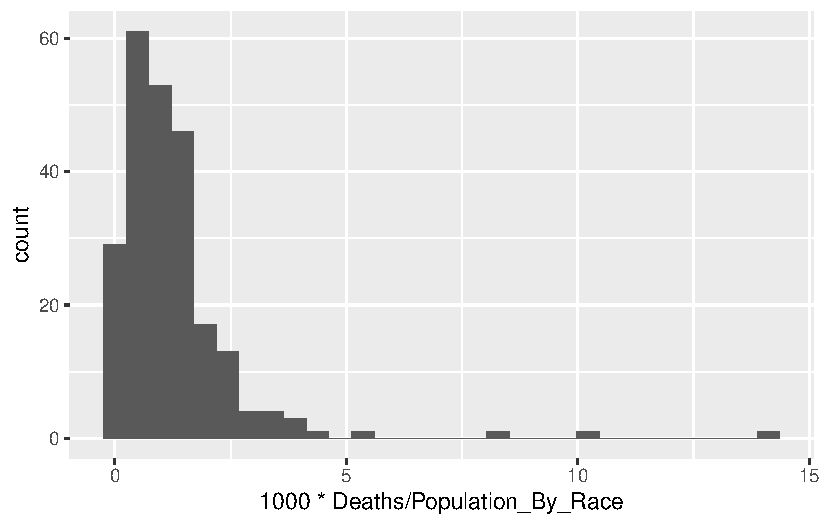
\includegraphics{StatsForFinalCSV_files/figure-pdf/unnamed-chunk-5-1.pdf}

\subsection{Fitting and analyzing a
model}\label{fitting-and-analyzing-a-model}

must set the baseline levels to compare to

\begin{Shaded}
\begin{Highlighting}[]
\NormalTok{covidna }\OtherTok{\textless{}{-}}\NormalTok{ covidna}\SpecialCharTok{|\textgreater{}}
  \FunctionTok{mutate}\NormalTok{(}\AttributeTok{Race =} \FunctionTok{relevel}\NormalTok{(}\FunctionTok{factor}\NormalTok{(Race), }\AttributeTok{ref =} \StringTok{"White"}\NormalTok{))}
\NormalTok{covidna }\OtherTok{\textless{}{-}}\NormalTok{ covidna}\SpecialCharTok{|\textgreater{}}
  \FunctionTok{mutate}\NormalTok{(}\AttributeTok{Gov\_Control =} \FunctionTok{relevel}\NormalTok{(}\FunctionTok{factor}\NormalTok{(Gov\_Control), }\AttributeTok{ref =} \StringTok{"Red"}\NormalTok{))}
\NormalTok{covidna }\OtherTok{\textless{}{-}}\NormalTok{ covidna}\SpecialCharTok{|\textgreater{}}
  \FunctionTok{mutate}\NormalTok{(}\AttributeTok{Region =} \FunctionTok{relevel}\NormalTok{(}\FunctionTok{factor}\NormalTok{(Region), }\AttributeTok{ref =} \StringTok{"Northeast"}\NormalTok{))}
\end{Highlighting}
\end{Shaded}

\begin{Shaded}
\begin{Highlighting}[]
\NormalTok{model\_beta }\OtherTok{\textless{}{-}} \FunctionTok{betareg}\NormalTok{(death\_rate\_prop }\SpecialCharTok{\textasciitilde{}}\NormalTok{ Race}\SpecialCharTok{+}\NormalTok{Gov\_Control}\SpecialCharTok{+}\NormalTok{Region, }\AttributeTok{data =}\NormalTok{ covidna)}
\FunctionTok{summary}\NormalTok{(model\_beta)}
\end{Highlighting}
\end{Shaded}

\begin{verbatim}

Call:
betareg(formula = death_rate_prop ~ Race + Gov_Control + Region, data = covidna)

Quantile residuals:
    Min      1Q  Median      3Q     Max 
-3.1370 -0.5002 -0.0806  0.3629  5.4567 

Coefficients (mean model with logit link):
                    Estimate Std. Error z value Pr(>|z|)    
(Intercept)        -6.555597   0.170129 -38.533  < 2e-16 ***
RaceAIAN            0.293952   0.153727   1.912 0.055854 .  
RaceAsian          -0.478085   0.136091  -3.513 0.000443 ***
RaceBlack          -0.030232   0.123184  -0.245 0.806129    
RaceMultiracial    -1.296711   0.250529  -5.176 2.27e-07 ***
RaceNHPI            0.532099   0.318884   1.669 0.095192 .  
RaceOther          -0.438776   0.135841  -3.230 0.001238 ** 
Gov_ControlBlue    -0.008681   0.127522  -0.068 0.945729    
Gov_ControlDivided -0.026301   0.117851  -0.223 0.823402    
RegionMidatlantic   0.056811   0.179548   0.316 0.751693    
RegionMidwest       0.243234   0.163726   1.486 0.137382    
RegionPacific      -0.440964   0.183123  -2.408 0.016039 *  
RegionSouth         0.207406   0.172673   1.201 0.229694    
RegionWest          0.016221   0.162292   0.100 0.920386    

Phi coefficients (precision model with identity link):
      Estimate Std. Error z value Pr(>|z|)    
(phi)   1369.4      136.5   10.03   <2e-16 ***
---
Signif. codes:  0 '***' 0.001 '**' 0.01 '*' 0.05 '.' 0.1 ' ' 1 

Type of estimator: ML (maximum likelihood)
Log-likelihood:  1377 on 15 Df
Pseudo R-squared: 0.3409
Number of iterations: 63 (BFGS) + 5 (Fisher scoring) 
\end{verbatim}

\begin{Shaded}
\begin{Highlighting}[]
\FunctionTok{exp}\NormalTok{(}\FunctionTok{coef}\NormalTok{(model\_beta))}
\end{Highlighting}
\end{Shaded}

\begin{verbatim}
       (Intercept)           RaceAIAN          RaceAsian          RaceBlack 
       0.001422133        1.341719616        0.619969301        0.970220296 
   RaceMultiracial           RaceNHPI          RaceOther    Gov_ControlBlue 
       0.273429693        1.702501321        0.644825174        0.991356966 
Gov_ControlDivided  RegionMidatlantic      RegionMidwest      RegionPacific 
       0.974041904        1.058455304        1.275366648        0.643415560 
       RegionSouth         RegionWest              (phi) 
       1.230482136        1.016352981                Inf 
\end{verbatim}

\begin{Shaded}
\begin{Highlighting}[]
\CommentTok{\# Get marginal means (still on response scale)}
\NormalTok{race\_emm }\OtherTok{\textless{}{-}} \FunctionTok{emmeans}\NormalTok{(model\_beta, }\SpecialCharTok{\textasciitilde{}}\NormalTok{ Race)}
\CommentTok{\# Get confidence intervals on response scale}
\NormalTok{race\_ci }\OtherTok{\textless{}{-}} \FunctionTok{confint}\NormalTok{(race\_emm, }\AttributeTok{type =} \StringTok{"response"}\NormalTok{)}\SpecialCharTok{|\textgreater{}}
  \FunctionTok{as.data.frame}\NormalTok{()}
\CommentTok{\# Check to verify:}
\FunctionTok{names}\NormalTok{(race\_ci)}
\end{Highlighting}
\end{Shaded}

\begin{verbatim}
[1] "Race"      "emmean"    "SE"        "df"        "asymp.LCL" "asymp.UCL"
\end{verbatim}

\begin{Shaded}
\begin{Highlighting}[]
\CommentTok{\# Get compact letter display (still from response{-}scale estimates)}
\NormalTok{race\_cld }\OtherTok{\textless{}{-}} \FunctionTok{cld}\NormalTok{(race\_emm, }\AttributeTok{Letters =}\NormalTok{ letters, }\AttributeTok{type =} \StringTok{"response"}\NormalTok{)}

\CommentTok{\# Merge group letters into CI data}
\NormalTok{race\_df }\OtherTok{\textless{}{-}}\NormalTok{ race\_ci }\SpecialCharTok{\%\textgreater{}\%}
  \FunctionTok{left\_join}\NormalTok{(}\FunctionTok{select}\NormalTok{(}\FunctionTok{as.data.frame}\NormalTok{(race\_cld), Race, .group), }\AttributeTok{by =} \StringTok{"Race"}\NormalTok{)}

\CommentTok{\# Plot}
\FunctionTok{ggplot}\NormalTok{(race\_df, }\FunctionTok{aes}\NormalTok{(}\AttributeTok{x =} \FunctionTok{reorder}\NormalTok{(Race, emmean), }\AttributeTok{y =}\NormalTok{ emmean)) }\SpecialCharTok{+}
  \FunctionTok{geom\_col}\NormalTok{(}\AttributeTok{fill =} \StringTok{"\#56B4E9"}\NormalTok{, }\AttributeTok{width =} \FloatTok{0.6}\NormalTok{) }\SpecialCharTok{+}
  \FunctionTok{geom\_errorbar}\NormalTok{(}\FunctionTok{aes}\NormalTok{(}\AttributeTok{ymin =}\NormalTok{ asymp.LCL, }\AttributeTok{ymax =}\NormalTok{ asymp.UCL), }\AttributeTok{width =} \FloatTok{0.2}\NormalTok{) }\SpecialCharTok{+}
  \FunctionTok{geom\_text}\NormalTok{(}\FunctionTok{aes}\NormalTok{(}\AttributeTok{label =}\NormalTok{ .group), }\AttributeTok{vjust =} \SpecialCharTok{{-}}\FloatTok{0.5}\NormalTok{, }\AttributeTok{size =} \DecValTok{5}\NormalTok{, }\AttributeTok{fontface =} \StringTok{"bold"}\NormalTok{) }\SpecialCharTok{+}
  \FunctionTok{labs}\NormalTok{(}
    \AttributeTok{title =} \StringTok{"Estimated COVID{-}19 Death Proportion by Race"}\NormalTok{,}
    \AttributeTok{x =} \StringTok{"Race"}\NormalTok{,}
    \AttributeTok{y =} \StringTok{"Adjusted Proportion (with 95\% CI)"}
\NormalTok{  ) }\SpecialCharTok{+}
  \FunctionTok{theme\_bw}\NormalTok{()}
\end{Highlighting}
\end{Shaded}

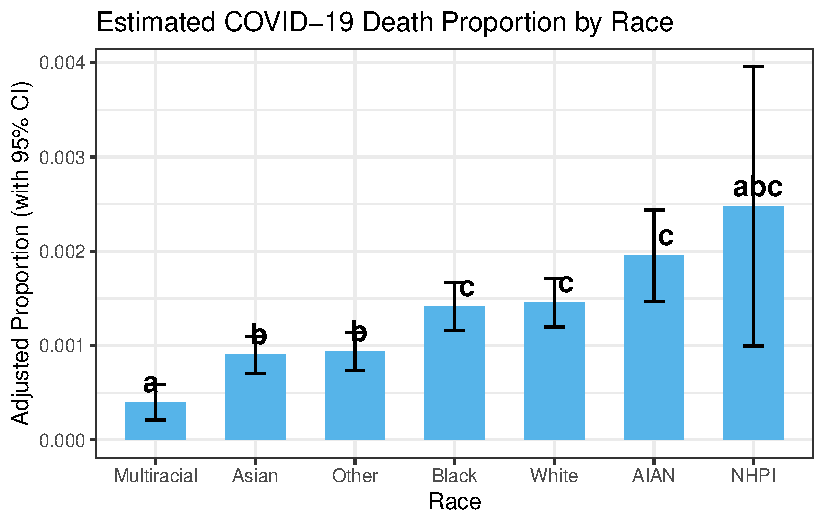
\includegraphics{StatsForFinalCSV_files/figure-pdf/unnamed-chunk-9-1.pdf}

\begin{Shaded}
\begin{Highlighting}[]
\CommentTok{\#ggsave("EstDeathRate.jpg",width = 10,height = 6)}

\NormalTok{covidnasum1}\OtherTok{\textless{}{-}}\NormalTok{covidna}\SpecialCharTok{|\textgreater{}}
  \FunctionTok{group\_by}\NormalTok{(Race)}\SpecialCharTok{|\textgreater{}}
  \FunctionTok{summarize}\NormalTok{(}\AttributeTok{total\_death\_rate=}\FunctionTok{sum}\NormalTok{(Deaths)}\SpecialCharTok{/}\FunctionTok{sum}\NormalTok{(Population\_By\_Race))}
\FunctionTok{ggplot}\NormalTok{(covidnasum1,}\FunctionTok{aes}\NormalTok{(}\FunctionTok{factor}\NormalTok{(Race,}\AttributeTok{levels =} \FunctionTok{c}\NormalTok{(}\StringTok{"Multiracial"}\NormalTok{,}\StringTok{"Asian"}\NormalTok{,}\StringTok{"Other"}\NormalTok{,}\StringTok{"Black"}\NormalTok{,}\StringTok{"White"}\NormalTok{,}\StringTok{"AIAN"}\NormalTok{,}\StringTok{"NHPI"}\NormalTok{)),}\DecValTok{1000}\SpecialCharTok{*}\NormalTok{total\_death\_rate))}\SpecialCharTok{+}
  \FunctionTok{geom\_col}\NormalTok{(}\AttributeTok{fill =} \StringTok{"\#56B4E9"}\NormalTok{, }\AttributeTok{width =} \FloatTok{0.6}\NormalTok{)}\SpecialCharTok{+}
  \FunctionTok{labs}\NormalTok{(}\AttributeTok{x=}\StringTok{"Race"}\NormalTok{,}\AttributeTok{title =} \StringTok{"Overall Death per 1000 Rate by Race"}\NormalTok{)}\SpecialCharTok{+}\FunctionTok{theme\_bw}\NormalTok{()}
\end{Highlighting}
\end{Shaded}

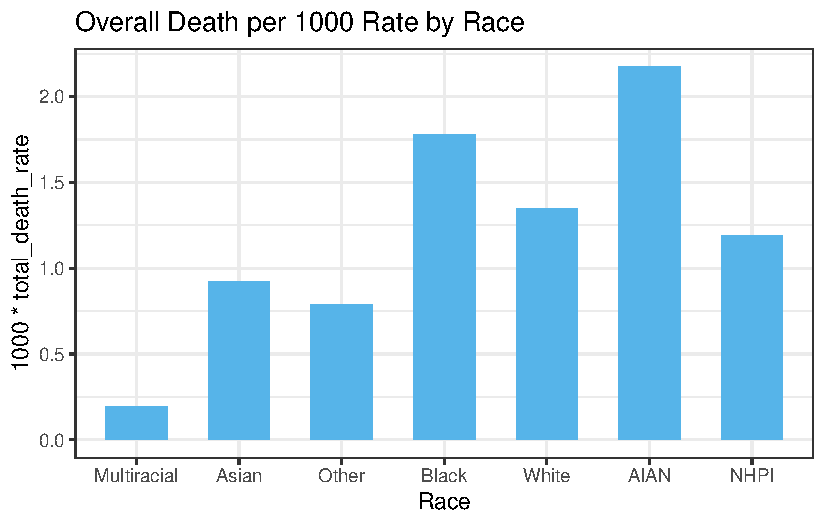
\includegraphics{StatsForFinalCSV_files/figure-pdf/unnamed-chunk-9-2.pdf}

\begin{Shaded}
\begin{Highlighting}[]
\CommentTok{\#ggsave("RealDeathProp.jpg",width = 10,height = 6)}
\end{Highlighting}
\end{Shaded}

\begin{Shaded}
\begin{Highlighting}[]
\CommentTok{\# Get marginal means by Race × Gov\_Control × Region}
\NormalTok{emm\_race\_full }\OtherTok{\textless{}{-}} \FunctionTok{emmeans}\NormalTok{(model\_beta, }\SpecialCharTok{\textasciitilde{}}\NormalTok{ Race }\SpecialCharTok{|}\NormalTok{ Gov\_Control }\SpecialCharTok{*}\NormalTok{ Region)}
\CommentTok{\# Convert to data frame with CIs}
\NormalTok{race\_ci }\OtherTok{\textless{}{-}} \FunctionTok{confint}\NormalTok{(emm\_race\_full, }\AttributeTok{type =} \StringTok{"response"}\NormalTok{)}\SpecialCharTok{|\textgreater{}}
  \FunctionTok{as.data.frame}\NormalTok{()}
\CommentTok{\# Significance groups per panel (Gov\_Control × Region)}
\NormalTok{race\_cld }\OtherTok{\textless{}{-}} \FunctionTok{cld}\NormalTok{(emm\_race\_full, }\AttributeTok{Letters =}\NormalTok{ letters, }\AttributeTok{type =} \StringTok{"response"}\NormalTok{)}
\CommentTok{\# Merge group letters into CI data}
\NormalTok{race\_df }\OtherTok{\textless{}{-}}\NormalTok{ race\_ci }\SpecialCharTok{\%\textgreater{}\%}
  \FunctionTok{left\_join}\NormalTok{(}\FunctionTok{select}\NormalTok{(}\FunctionTok{as.data.frame}\NormalTok{(race\_cld), Race, Gov\_Control, Region, .group),}
            \AttributeTok{by =} \FunctionTok{c}\NormalTok{(}\StringTok{"Race"}\NormalTok{, }\StringTok{"Gov\_Control"}\NormalTok{, }\StringTok{"Region"}\NormalTok{))}
\FunctionTok{ggplot}\NormalTok{(race\_df, }\FunctionTok{aes}\NormalTok{(}\AttributeTok{x =} \FunctionTok{reorder}\NormalTok{(Race, emmean), }\AttributeTok{y =}\NormalTok{ emmean)) }\SpecialCharTok{+}
  \FunctionTok{geom\_col}\NormalTok{(}\AttributeTok{fill =} \StringTok{"\#56B4E9"}\NormalTok{, }\AttributeTok{width =} \FloatTok{0.6}\NormalTok{) }\SpecialCharTok{+}
  \FunctionTok{geom\_errorbar}\NormalTok{(}\FunctionTok{aes}\NormalTok{(}\AttributeTok{ymin =}\NormalTok{ asymp.LCL, }\AttributeTok{ymax =}\NormalTok{ asymp.UCL), }\AttributeTok{width =} \FloatTok{0.2}\NormalTok{) }\SpecialCharTok{+}
  \FunctionTok{geom\_text}\NormalTok{(}\FunctionTok{aes}\NormalTok{(}\AttributeTok{label =}\NormalTok{ .group), }\AttributeTok{vjust =} \SpecialCharTok{{-}}\FloatTok{0.5}\NormalTok{, }\AttributeTok{size =} \FloatTok{4.5}\NormalTok{, }\AttributeTok{fontface =} \StringTok{"bold"}\NormalTok{) }\SpecialCharTok{+}
  \FunctionTok{facet\_grid}\NormalTok{(Region }\SpecialCharTok{\textasciitilde{}}\NormalTok{ Gov\_Control) }\SpecialCharTok{+}  \CommentTok{\# Facet by Region (rows) and Gov\_Control (columns)}
  \FunctionTok{labs}\NormalTok{(}
    \AttributeTok{title =} \StringTok{"Adjusted COVID{-}19 Death Proportion by Race, Region, and Government Control"}\NormalTok{,}
    \AttributeTok{x =} \StringTok{"Race"}\NormalTok{,}
    \AttributeTok{y =} \StringTok{"Estimated Proportion (with 95\% CI)"}
\NormalTok{  ) }\SpecialCharTok{+}
  \FunctionTok{theme\_minimal}\NormalTok{(}\AttributeTok{base\_size =} \DecValTok{13}\NormalTok{) }\SpecialCharTok{+}
  \FunctionTok{theme}\NormalTok{(}
    \AttributeTok{axis.text.x =} \FunctionTok{element\_text}\NormalTok{(}\AttributeTok{angle =} \DecValTok{45}\NormalTok{, }\AttributeTok{hjust =} \DecValTok{1}\NormalTok{),}
    \AttributeTok{strip.text =} \FunctionTok{element\_text}\NormalTok{(}\AttributeTok{face =} \StringTok{"bold"}\NormalTok{)}
\NormalTok{  )}
\end{Highlighting}
\end{Shaded}

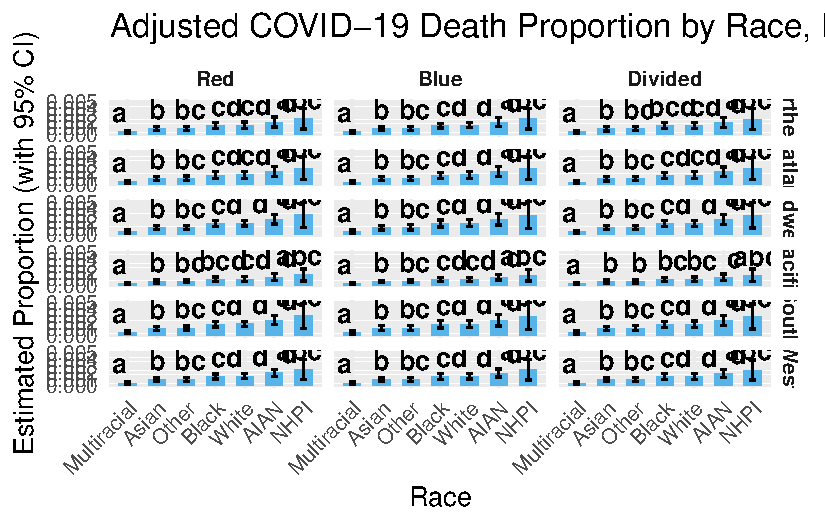
\includegraphics{StatsForFinalCSV_files/figure-pdf/unnamed-chunk-10-1.pdf}

\subsection{Setting up for our model}\label{setting-up-for-our-model-1}

Taking out super low proportions due to skewing caused by such low
numbers, also taking zeros out.

\begin{Shaded}
\begin{Highlighting}[]
\NormalTok{covidnacase}\OtherTok{\textless{}{-}}\NormalTok{covid1}\SpecialCharTok{|\textgreater{}}
  \FunctionTok{filter}\NormalTok{(}\SpecialCharTok{!}\FunctionTok{is.na}\NormalTok{(Cases))}\SpecialCharTok{|\textgreater{}}
  \FunctionTok{filter}\NormalTok{(Cases}\SpecialCharTok{\textgreater{}}\DecValTok{0}\NormalTok{)}
\NormalTok{covidnacase}\OtherTok{\textless{}{-}}\NormalTok{covidnacase}\SpecialCharTok{|\textgreater{}}
  \FunctionTok{mutate}\NormalTok{(}\AttributeTok{case\_rate\_prop =}\NormalTok{ Cases }\SpecialCharTok{/}\NormalTok{ Population\_By\_Race)}
\NormalTok{covidnacase}\OtherTok{\textless{}{-}}\NormalTok{covidnacase}\SpecialCharTok{|\textgreater{}}
  \FunctionTok{filter}\NormalTok{(Race\_Proportion}\SpecialCharTok{\textgreater{}=}\FloatTok{0.005}\NormalTok{)}
\end{Highlighting}
\end{Shaded}

\subsection{Visualize distribution of death
rate}\label{visualize-distribution-of-death-rate-1}

\begin{Shaded}
\begin{Highlighting}[]
\FunctionTok{ggplot}\NormalTok{(covidnacase,}\FunctionTok{aes}\NormalTok{(}\DecValTok{1000}\SpecialCharTok{*}\NormalTok{Cases}\SpecialCharTok{/}\NormalTok{Population\_By\_Race))}\SpecialCharTok{+}
  \FunctionTok{geom\_histogram}\NormalTok{()}
\end{Highlighting}
\end{Shaded}

\begin{verbatim}
`stat_bin()` using `bins = 30`. Pick better value with `binwidth`.
\end{verbatim}

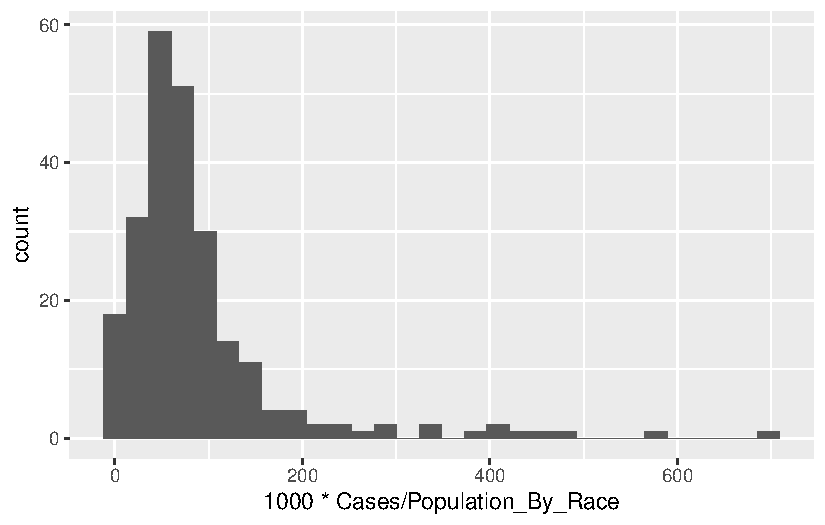
\includegraphics{StatsForFinalCSV_files/figure-pdf/unnamed-chunk-12-1.pdf}

\subsection{Fitting and analyzing a
model}\label{fitting-and-analyzing-a-model-1}

must set the baseline levels to compare to

\begin{Shaded}
\begin{Highlighting}[]
\NormalTok{covidnacase }\OtherTok{\textless{}{-}}\NormalTok{ covidnacase}\SpecialCharTok{|\textgreater{}}
  \FunctionTok{mutate}\NormalTok{(}\AttributeTok{Race =} \FunctionTok{relevel}\NormalTok{(}\FunctionTok{factor}\NormalTok{(Race), }\AttributeTok{ref =} \StringTok{"White"}\NormalTok{))}
\NormalTok{covidnacase }\OtherTok{\textless{}{-}}\NormalTok{ covidnacase}\SpecialCharTok{|\textgreater{}}
  \FunctionTok{mutate}\NormalTok{(}\AttributeTok{Gov\_Control =} \FunctionTok{relevel}\NormalTok{(}\FunctionTok{factor}\NormalTok{(Gov\_Control), }\AttributeTok{ref =} \StringTok{"Red"}\NormalTok{))}
\NormalTok{covidnacase }\OtherTok{\textless{}{-}}\NormalTok{ covidnacase}\SpecialCharTok{|\textgreater{}}
  \FunctionTok{mutate}\NormalTok{(}\AttributeTok{Region =} \FunctionTok{relevel}\NormalTok{(}\FunctionTok{factor}\NormalTok{(Region), }\AttributeTok{ref =} \StringTok{"Northeast"}\NormalTok{))}
\end{Highlighting}
\end{Shaded}

\begin{Shaded}
\begin{Highlighting}[]
\NormalTok{model\_betacase }\OtherTok{\textless{}{-}} \FunctionTok{betareg}\NormalTok{(case\_rate\_prop }\SpecialCharTok{\textasciitilde{}}\NormalTok{ Race}\SpecialCharTok{+}\NormalTok{Gov\_Control}\SpecialCharTok{+}\NormalTok{Region, }\AttributeTok{data =}\NormalTok{ covidnacase)}
\FunctionTok{summary}\NormalTok{(model\_betacase)}
\end{Highlighting}
\end{Shaded}

\begin{verbatim}

Call:
betareg(formula = case_rate_prop ~ Race + Gov_Control + Region, data = covidnacase)

Quantile residuals:
    Min      1Q  Median      3Q     Max 
-5.0452 -0.3937 -0.0818  0.3009  4.7887 

Coefficients (mean model with logit link):
                   Estimate Std. Error z value Pr(>|z|)    
(Intercept)        -2.39794    0.19050 -12.588  < 2e-16 ***
RaceAIAN            0.45697    0.18058   2.531  0.01139 *  
RaceAsian          -0.12718    0.15485  -0.821  0.41147    
RaceBlack           0.20941    0.14672   1.427  0.15350    
RaceMultiracial    -0.71540    0.24308  -2.943  0.00325 ** 
RaceNHPI            0.92654    0.34262   2.704  0.00684 ** 
RaceOther           0.65742    0.14016   4.690 2.73e-06 ***
Gov_ControlBlue    -0.41119    0.13526  -3.040  0.00237 ** 
Gov_ControlDivided -0.03444    0.12552  -0.274  0.78378    
RegionMidatlantic   0.14957    0.19346   0.773  0.43944    
RegionMidwest       0.06751    0.17689   0.382  0.70270    
RegionPacific      -0.18543    0.19597  -0.946  0.34403    
RegionSouth        -0.10043    0.18934  -0.530  0.59582    
RegionWest          0.11553    0.17648   0.655  0.51271    

Phi coefficients (precision model with identity link):
      Estimate Std. Error z value Pr(>|z|)    
(phi)   17.822      1.698    10.5   <2e-16 ***
---
Signif. codes:  0 '***' 0.001 '**' 0.01 '*' 0.05 '.' 0.1 ' ' 1 

Type of estimator: ML (maximum likelihood)
Log-likelihood: 377.7 on 15 Df
Pseudo R-squared: 0.2992
Number of iterations: 23 (BFGS) + 1 (Fisher scoring) 
\end{verbatim}

\begin{Shaded}
\begin{Highlighting}[]
\FunctionTok{exp}\NormalTok{(}\FunctionTok{coef}\NormalTok{(model\_betacase))}
\end{Highlighting}
\end{Shaded}

\begin{verbatim}
       (Intercept)           RaceAIAN          RaceAsian          RaceBlack 
      9.090493e-02       1.579283e+00       8.805773e-01       1.232952e+00 
   RaceMultiracial           RaceNHPI          RaceOther    Gov_ControlBlue 
      4.889974e-01       2.525753e+00       1.929808e+00       6.628623e-01 
Gov_ControlDivided  RegionMidatlantic      RegionMidwest      RegionPacific 
      9.661434e-01       1.161336e+00       1.069844e+00       8.307448e-01 
       RegionSouth         RegionWest              (phi) 
      9.044484e-01       1.122470e+00       5.496396e+07 
\end{verbatim}

\begin{Shaded}
\begin{Highlighting}[]
\CommentTok{\# Get marginal means (still on response scale)}
\NormalTok{race\_emmcase }\OtherTok{\textless{}{-}} \FunctionTok{emmeans}\NormalTok{(model\_betacase, }\SpecialCharTok{\textasciitilde{}}\NormalTok{ Race)}
\CommentTok{\# Get confidence intervals on response scale}
\NormalTok{race\_cicase }\OtherTok{\textless{}{-}} \FunctionTok{confint}\NormalTok{(race\_emmcase, }\AttributeTok{type =} \StringTok{"response"}\NormalTok{)}\SpecialCharTok{|\textgreater{}}
  \FunctionTok{as.data.frame}\NormalTok{()}
\CommentTok{\# Check to verify:}
\FunctionTok{names}\NormalTok{(race\_cicase)}
\end{Highlighting}
\end{Shaded}

\begin{verbatim}
[1] "Race"      "emmean"    "SE"        "df"        "asymp.LCL" "asymp.UCL"
\end{verbatim}

\begin{Shaded}
\begin{Highlighting}[]
\CommentTok{\# Get compact letter display (still from response{-}scale estimates)}
\NormalTok{race\_cldcase }\OtherTok{\textless{}{-}} \FunctionTok{cld}\NormalTok{(race\_emmcase, }\AttributeTok{Letters =}\NormalTok{ letters, }\AttributeTok{type =} \StringTok{"response"}\NormalTok{)}

\CommentTok{\# Merge group letters into CI data}
\NormalTok{race\_dfcase }\OtherTok{\textless{}{-}}\NormalTok{ race\_cicase }\SpecialCharTok{\%\textgreater{}\%}
  \FunctionTok{left\_join}\NormalTok{(}\FunctionTok{select}\NormalTok{(}\FunctionTok{as.data.frame}\NormalTok{(race\_cldcase), Race, .group), }\AttributeTok{by =} \StringTok{"Race"}\NormalTok{)}

\CommentTok{\# Plot}
\FunctionTok{ggplot}\NormalTok{(race\_dfcase, }\FunctionTok{aes}\NormalTok{(}\AttributeTok{x =} \FunctionTok{factor}\NormalTok{(Race,}\AttributeTok{levels =} \FunctionTok{c}\NormalTok{(}\StringTok{"Multiracial"}\NormalTok{,}\StringTok{"Asian"}\NormalTok{,}\StringTok{"Other"}\NormalTok{,}\StringTok{"Black"}\NormalTok{,}\StringTok{"White"}\NormalTok{,}\StringTok{"AIAN"}\NormalTok{,}\StringTok{"NHPI"}\NormalTok{)), }\AttributeTok{y =}\NormalTok{ emmean)) }\SpecialCharTok{+}
  \FunctionTok{geom\_col}\NormalTok{(}\AttributeTok{fill =} \StringTok{"\#56B4E9"}\NormalTok{, }\AttributeTok{width =} \FloatTok{0.6}\NormalTok{) }\SpecialCharTok{+}
  \FunctionTok{geom\_errorbar}\NormalTok{(}\FunctionTok{aes}\NormalTok{(}\AttributeTok{ymin =}\NormalTok{ asymp.LCL, }\AttributeTok{ymax =}\NormalTok{ asymp.UCL), }\AttributeTok{width =} \FloatTok{0.2}\NormalTok{) }\SpecialCharTok{+}
  \FunctionTok{geom\_text}\NormalTok{(}\FunctionTok{aes}\NormalTok{(}\AttributeTok{label =}\NormalTok{ .group), }\AttributeTok{vjust =} \SpecialCharTok{{-}}\FloatTok{0.5}\NormalTok{, }\AttributeTok{size =} \DecValTok{5}\NormalTok{, }\AttributeTok{fontface =} \StringTok{"bold"}\NormalTok{) }\SpecialCharTok{+}
  \FunctionTok{labs}\NormalTok{(}
    \AttributeTok{title =} \StringTok{"Estimated COVID{-}19 Proportion of Cases by Race"}\NormalTok{,}
    \AttributeTok{x =} \StringTok{"Race"}\NormalTok{,}
    \AttributeTok{y =} \StringTok{"Adjusted Proportion (with 95\% CI)"}
\NormalTok{  ) }\SpecialCharTok{+}
  \FunctionTok{theme\_bw}\NormalTok{()}
\end{Highlighting}
\end{Shaded}

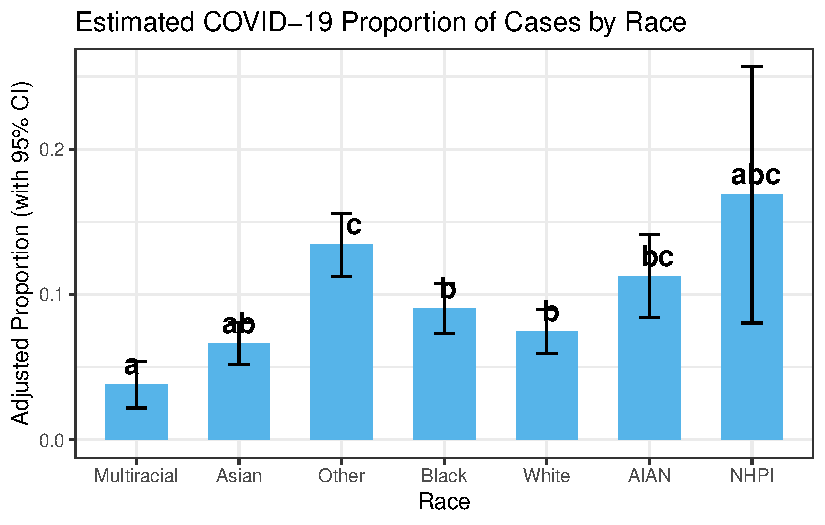
\includegraphics{StatsForFinalCSV_files/figure-pdf/unnamed-chunk-16-1.pdf}

\begin{Shaded}
\begin{Highlighting}[]
 \CommentTok{\# ggsave("EstCaseRate.jpg",width = 10,height = 6)}
\NormalTok{covidnasumcase}\OtherTok{\textless{}{-}}\NormalTok{covidnacase}\SpecialCharTok{|\textgreater{}}
  \FunctionTok{group\_by}\NormalTok{(Race)}\SpecialCharTok{|\textgreater{}}
  \FunctionTok{summarize}\NormalTok{(}\AttributeTok{total\_case\_rate=}\FunctionTok{sum}\NormalTok{(Cases)}\SpecialCharTok{/}\FunctionTok{sum}\NormalTok{(Population\_By\_Race))}
\FunctionTok{ggplot}\NormalTok{(covidnasumcase,}\FunctionTok{aes}\NormalTok{(}\FunctionTok{factor}\NormalTok{(Race,}\AttributeTok{levels =} \FunctionTok{c}\NormalTok{(}\StringTok{"Multiracial"}\NormalTok{,}\StringTok{"Asian"}\NormalTok{,}\StringTok{"Other"}\NormalTok{,}\StringTok{"Black"}\NormalTok{,}\StringTok{"White"}\NormalTok{,}\StringTok{"AIAN"}\NormalTok{,}\StringTok{"NHPI"}\NormalTok{)),}\DecValTok{1000}\SpecialCharTok{*}\NormalTok{total\_case\_rate))}\SpecialCharTok{+}
  \FunctionTok{geom\_col}\NormalTok{(}\AttributeTok{fill =} \StringTok{"\#56B4E9"}\NormalTok{, }\AttributeTok{width =} \FloatTok{0.6}\NormalTok{)}\SpecialCharTok{+}
  \FunctionTok{labs}\NormalTok{(}\AttributeTok{x=}\StringTok{"Race"}\NormalTok{,}\AttributeTok{title =} \StringTok{"Overall Case Rate per 1000 by Race"}\NormalTok{)}\SpecialCharTok{+}\FunctionTok{theme\_bw}\NormalTok{()}
\end{Highlighting}
\end{Shaded}

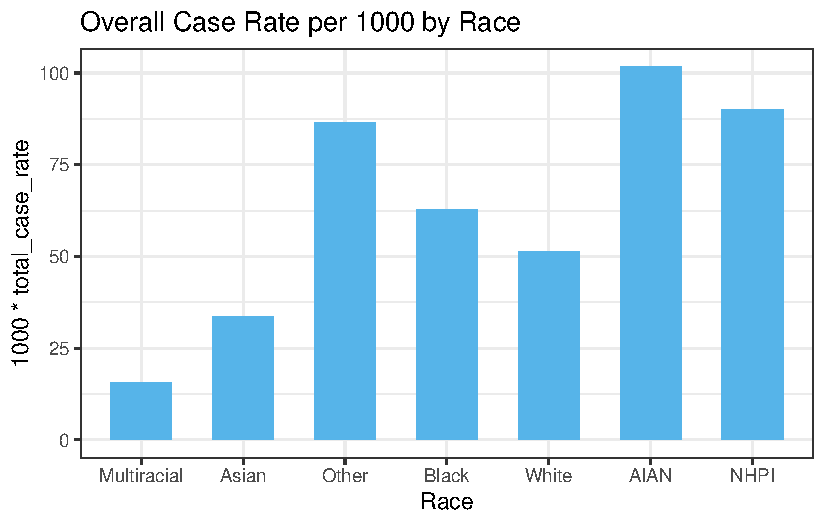
\includegraphics{StatsForFinalCSV_files/figure-pdf/unnamed-chunk-16-2.pdf}

\begin{Shaded}
\begin{Highlighting}[]
\CommentTok{\#ggsave("RealCaseProp.jpg",width = 10,height = 6)}
\end{Highlighting}
\end{Shaded}

\begin{Shaded}
\begin{Highlighting}[]
\NormalTok{emm\_race\_fullcase }\OtherTok{\textless{}{-}} \FunctionTok{emmeans}\NormalTok{(model\_betacase, }\SpecialCharTok{\textasciitilde{}}\NormalTok{ Race }\SpecialCharTok{|}\NormalTok{ Gov\_Control }\SpecialCharTok{*}\NormalTok{ Region)}
\NormalTok{race\_cicase }\OtherTok{\textless{}{-}} \FunctionTok{confint}\NormalTok{(emm\_race\_fullcase, }\AttributeTok{type =} \StringTok{"response"}\NormalTok{)}\SpecialCharTok{|\textgreater{}}
  \FunctionTok{as.data.frame}\NormalTok{()}
\NormalTok{race\_cldcase }\OtherTok{\textless{}{-}} \FunctionTok{cld}\NormalTok{(emm\_race\_fullcase, }\AttributeTok{Letters =}\NormalTok{ letters, }\AttributeTok{type =} \StringTok{"response"}\NormalTok{)}
\NormalTok{race\_dfcase }\OtherTok{\textless{}{-}}\NormalTok{ race\_cicase }\SpecialCharTok{\%\textgreater{}\%}
  \FunctionTok{left\_join}\NormalTok{(}\FunctionTok{select}\NormalTok{(}\FunctionTok{as.data.frame}\NormalTok{(race\_cldcase), Race, Gov\_Control, Region, .group),}
            \AttributeTok{by =} \FunctionTok{c}\NormalTok{(}\StringTok{"Race"}\NormalTok{, }\StringTok{"Gov\_Control"}\NormalTok{, }\StringTok{"Region"}\NormalTok{))}
\FunctionTok{ggplot}\NormalTok{(race\_dfcase, }\FunctionTok{aes}\NormalTok{(}\AttributeTok{x =} \FunctionTok{reorder}\NormalTok{(Race, emmean), }\AttributeTok{y =}\NormalTok{ emmean)) }\SpecialCharTok{+}
  \FunctionTok{geom\_col}\NormalTok{(}\AttributeTok{fill =} \StringTok{"\#56B4E9"}\NormalTok{, }\AttributeTok{width =} \FloatTok{0.6}\NormalTok{) }\SpecialCharTok{+}
  \FunctionTok{geom\_errorbar}\NormalTok{(}\FunctionTok{aes}\NormalTok{(}\AttributeTok{ymin =}\NormalTok{ asymp.LCL, }\AttributeTok{ymax =}\NormalTok{ asymp.UCL), }\AttributeTok{width =} \FloatTok{0.2}\NormalTok{) }\SpecialCharTok{+}
  \FunctionTok{geom\_text}\NormalTok{(}\FunctionTok{aes}\NormalTok{(}\AttributeTok{label =}\NormalTok{ .group), }\AttributeTok{vjust =} \SpecialCharTok{{-}}\FloatTok{0.5}\NormalTok{, }\AttributeTok{size =} \FloatTok{4.5}\NormalTok{, }\AttributeTok{fontface =} \StringTok{"bold"}\NormalTok{) }\SpecialCharTok{+}
  \FunctionTok{facet\_grid}\NormalTok{(Region }\SpecialCharTok{\textasciitilde{}}\NormalTok{ Gov\_Control) }\SpecialCharTok{+}  
  \FunctionTok{labs}\NormalTok{(}
    \AttributeTok{title =} \StringTok{"Adjusted COVID{-}19 Case Proportion by Race, Region, and Government Control"}\NormalTok{,}
    \AttributeTok{x =} \StringTok{"Race"}\NormalTok{,}
    \AttributeTok{y =} \StringTok{"Estimated Proportion (with 95\% CI)"}
\NormalTok{  ) }\SpecialCharTok{+}
  \FunctionTok{theme\_minimal}\NormalTok{(}\AttributeTok{base\_size =} \DecValTok{13}\NormalTok{) }\SpecialCharTok{+}
  \FunctionTok{theme}\NormalTok{(}
    \AttributeTok{axis.text.x =} \FunctionTok{element\_text}\NormalTok{(}\AttributeTok{angle =} \DecValTok{45}\NormalTok{, }\AttributeTok{hjust =} \DecValTok{1}\NormalTok{),}
    \AttributeTok{strip.text =} \FunctionTok{element\_text}\NormalTok{(}\AttributeTok{face =} \StringTok{"bold"}\NormalTok{)}
\NormalTok{  )}
\end{Highlighting}
\end{Shaded}

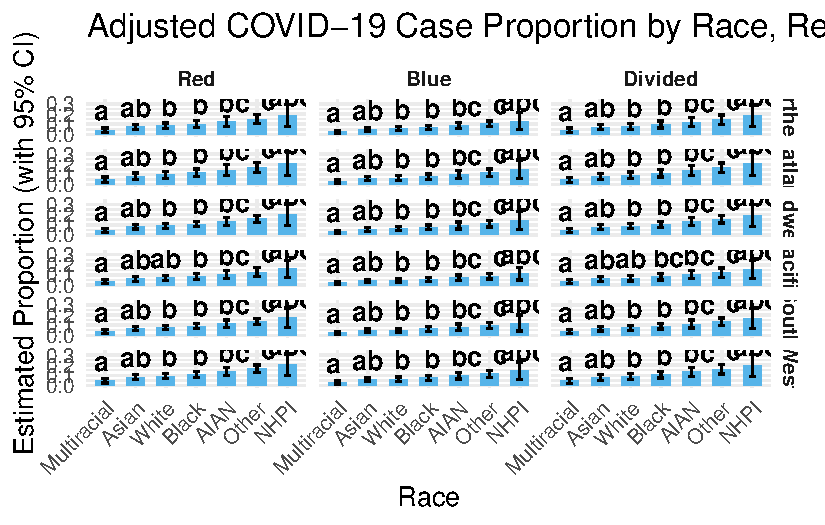
\includegraphics{StatsForFinalCSV_files/figure-pdf/unnamed-chunk-17-1.pdf}




\end{document}
